\RequirePackage{fix-cm}

\documentclass[twocolumn]{svjour3} 
\usepackage[utf8]{inputenc}
\usepackage[english]{babel}
\usepackage{letltxmacro}
\usepackage{graphicx}

\makeatother

\LetLtxMacro{\ORIGselectlanguage}{\selectlanguage}
\makeatletter
\DeclareRobustCommand{\selectlanguage}[1]{%
  \@ifundefined{alias@\string#1}
    {\ORIGselectlanguage{#1}}
    {\begingroup\edef\x{\endgroup
       \noexpand\ORIGselectlanguage{\@nameuse{alias@#1}}}\x}%
}
\newcommand{\definelanguagealias}[2]{%
  \@namedef{alias@#1}{#2}%
}
\makeatother

\definelanguagealias{eng}{english}
\definelanguagealias{en}{english}

\makeatletter
\let\l@eng\l@english
\makeatother

\usepackage{letltxmacro}

\usepackage{stringenc}
\usepackage{pdfescape}
\usepackage{subcaption}

\usepackage{url,hyperref,lineno,microtype}
\usepackage{mathptmx}

\hyphenation{da-ta-base da-ta-bases ex-pla-na-to-ry ex-plo-ra-to-ry}

\journalname{The Visual Computer}

\begin{document}

\title{A Multi-facetted Visual Analytics Tool for Exploratory Analysis of Human Brain and Function Datasets} 

\author{Diego Angulo \and Jose Hernandez \and James Oliver \and Cyril Schneider \and Nathalie Charpak}

\institute{Diego A. Angulo \and Jose T. Hernandez
\at IMAGINE, Systems and Computing Engineering, Universidad de los Andes, Carrera 1 \# 18A -12 , Bogota, Colombia
\email{da.angulo39@uniandes.edu.co} 
\and
James H. Oliver
\at VRAC, Iowa State University, Ames , IA, Unites States
\and
Cyril Schneider
\at CNS, CHUL, Quebec , QC, Canada 
\and 
Nathalie Charpak
\at Kangaroo Foundation, Bogota, Colombia
}


\maketitle


\begin{abstract}
Brain research typically requires large amounts of data from different sources and often, of different nature. The use of different software tools adapted to the nature of each data source can make research work cumbersome and time consuming. It follows that data is not often used to its fullest potential thus limiting exploratory analysis. This paper presents an ancillary software tool called BRAVIZ that integrates interactive visualization with real-time statistical analyses, facilitating access to multi-facetted neuroscience data and automating many cumbersome and error-prone tasks required to explore such data. Rather than relying on abstract numerical indicators, BRAVIZ emphasizes brain images as the main object of the analysis process of individuals or groups. BRAVIZs facilitates exploration of trends or relationships to gain an integrated view of the phenomena studied, thus motivating discovery of new hypotheses. A case study is presented that incorporates brain structure and function outcomes together with different types of clinical data.

\keywords{ Exploratory Analysis \and Visual Analytics \and Brain Data \and MRI \and Tractography \and Cohorts }
\end{abstract}

\section{Motivation}


An important challenge in brain research, in both normal and pathological conditions, is to better understand the extent to which the physical structure of brain underlies the way it functions. The most common research procedure is characterized by experiments aimed at collecting data directed towards testing a former hypothesis. This confirmatory-like methodology imposes limitations on the way data is used, and it is typically used only once which is unfortunate since data acquisition is generally time and resource intensive.


In the last two decades brain research data has increasingly been gathered in a more open fashion and many databases are now available to the public \cite{milham_open_2012}. In parallel, improvements in data collection, storage and sharing, at both technical and policy levels, have advanced \cite{eckersley_neuroscience_2003}, together with technologies to consolidate, search and access the data \cite{van_horn_is_2009,wood_harnessing_2014}. This allows massive amounts of data to be consolidated into databases and searched in efficient ways. In this way questions can be explored and large data pools can be mined for interesting relationships.




This has led to rapid changes in the way research can be conducted, i.e., a shift from hypothesis-driven research into data-driven research, where data is available first and research questions and hypotheses are formulated on the basis of the exploration of data. The methodology used in data-driven research differs significantly from that for hypothesis-driven research. Data driven research seeks to find and extract meaningful insights from data using exploratory research \cite{tukey_we_1980} and has already proven efficiency in economics, terrorism prevention and business intelligence domains which are characterized by large and heterogeneous data sets \cite{cook_illuminating_2005}. Exploratory research involves iterating through data several times, looking at it from different points of view, transforming data, searching for interesting subjects and measurements, gathering details and performing group analyses. These analysis tasks are carried out multiple times, and often in different order, as researchers learn more about the data. It is therefore helpful to provide tools to make annotations and save findings, so that explorations can be continued later.


During this process several data patterns may likely lead to unexpected insights. Unfortunately, it is also likely that these patterns are caused by the unique noise structure of the current data and therefore cannot be generalized to the global population. Automatic data-mining algorithms can find thousands of possible relations, but true findings need to be backed up by science and current knowledge.  Therefore, domain experts must be involved in interpretation of insights. Moreover, insights that integrate data from different domains require experts from all these domains.


Visual analytics \cite{keim_visual_2008} has emerged as a discipline that seeks to integrate statistics, machine learning, data mining and interactive data visualization with the objective of optimizing the use of data available for exploratory research. The analyst is acknowledged as the most important actor, and all tools are designed to support exploration and provide timely access to the required data as well as to informatics and statistics functions. Another principle in visual analytics is that analysts should focus on data and not on operational details of the tools. Therefore tools should provide the data and functionality to complete the task, while keeping non-relevant details and complex functionality hidden.

Exploratory brain research is a domain that could certainly benefit from visual analytics techniques. Indeed, brain function-related datasets are a combination of spatial (brain imaging) and non-spatial (clinical) measurements that could be analyzed together to better understand the link between brain structure and function as they relate to human health and behavior. Examples of spatial measurements include brain anatomy acquired by means of magnetic resonance imaging (MRI), neural pathways trajectory acquired by diffusion weighted imaging (DWI) or patterns of cerebral activation in specific tasks and acquired by functional MRI (fMRI). Specialized tools can process these imaging modalities to model brain structure, build pathways, produce statistical maps of activation patterns and neural connections. Brain researchers need to correlate these measurements and models to data of a different nature, such as neuropsychological performance and other clinical data.


However, the tools currently used in brain research are generally specific to the type or domain of data analyzed and they are optimized to support linear work flows. It follows that experts must often switch between tools to integrate and analyze data from different domains. In the worst cases, they may even have to move to a different computer. This process is time-consuming and repetitive. It requires the analyst to focus attention on the ``how'' rather than the ``what'', and thus makes exploratory analysis challenging.
					
\section{Introduction}

This paper introduces BRAVIZ, a software tool based on visual analytics and aimed at supporting exploratory analysis in brain research. More specifically, it is a tool focused on datasets that include MRI derived measurements and models 
as well as clinical outcomes. BRAVIZ is comprised of several applications that integrate interactive visualizations, links to detailed meta-data, creation of new variables as well as statistical models and analyses -  all of which are designed to support and facilitate full exploratory analyses.

\section{Related Work on Neuroimaging and Exploratory Analysis}


Several tools can already be used by visual analytics applications to support research on neuroimaging. For example, Freesurfer \cite{fischl_freesurfer_2012}, FSL \cite{jenkinson_fsl_2012} and SPM \cite{friston_statistical_2006} segment, register and perform statistical testing of brain image data. 3D Slicer \cite{fedorov_3d_2012}, Brain Visa \cite{cointepas_brainvisa:_2001} and ITKSnap \cite{yushkevich_user-guided_2006} are commonly used to integrate data from different image modalities (structural, diffusion-weighted, functional among others). They have all proven to be efficient at processing bulk images in a pipeline, and visualizing data from a single subject, but they fall short when several iterations through the data are required. The interfaces proposed for statistical testing require extensive configuration, which is appropriate for testing specific hypotheses, but become cumbersome when several possibilities are to be explored. Efficient mechanisms for restricting analysis to only a set of subjects or going back to a subject's details are missing. Complementary data loaded from tables can be used, but changing variables often means creating new tables and making them fit the requested format.


Non-spatial information visualization tools like GGobi \cite{cook_interactive_2007}, and Tableau\cite{hanrahan_tableau_2003} can be used for interactive exploratory analysis. They support data transformations, model fitting, and interactive visualization. They also enable  detection of outliers (important in data-driven research whereas usually removed from hypothesis-driven research), provide additional details, determine subgroups, and visualize patterns and trends in different ways (e.g. parallel coordinates, scatter plots, histograms, etc). However, these tools do not integrate well with spatial data. Scalar data derived from original images can be added but there is no easy way to link back to the original data or to explore spatial features that cannot be encoded into numerical variables.

INVIZIAN \cite{bowman_query-based_2011,bowman_feature-similarity_2012,bowman_visual_2012} uses GGobi options to explore, in an abstract 3D space, the relations between scalar values and anatomical features of large brain datasets. It provides an environment for exploratory research involving data from several databases and is targeted toward hypotheses generation. However, it works only with automatic feature extraction from structural MRI. INVIZIAN shares one common goal with BRAVIZ in that it focuses on easing the users visual pattern search. However, BRAVIZ supports a variety of different types of imaging data, from structural to functional MRI for example, and focuses on facilitating interpretation of data generated by users rather than on machine learning.


INVIZIAN \cite{bowman_query-based_2011}\cite{bowman_feature-similarity_2012}\cite{bowman_visual_2012} uses ggobi options to explore in an abstract 3D space the relations between scalar values and anatomical features of large brain datasets. It provides an environment for exploratory research involving data from several databases targeted to hypotheses generation. However, it only works with automatic feature extraction from structural MRI. As BRAVIZ, INVIZIAN focuses on easing the user’s visual pattern search, but BRAVIZ targets projects including the analysis of different types of data from structural to functional MRI for example, and focuses on data generated by users rather than on machine learning. 


A visual analysis tool for high dimensional genetic and clinical data is presented in \cite{hinterberg_peax:_2014}. The user explores the data by quickly iterating through several models that relate genetic data to clinical outcomes. Models are displayed as trees and linked with distributions of the selected parameters. Tools are provided to automatically find the most relevant parameters therefore reducing the search space. This tool is optimized for a single type of data, a single type of model and a specific workflow. In contrast, BRAVIZ seeks to support multiple tasks, data types and workflows by providing a set of  applications to be used independently or combined for complex exploratory analyses.
	
Even though multiple tools  exist for analysis and exploration of spatial and non-spatial data, the integration of multiple kinds/levels of analyses and data in a single environment remains challenging. BRAVIZ provides a unique unified environment for analyzing spatial and non-spatial data interactively, and in this way, it supports data-driven research.

\section{The BRAVIZ Proposal}

Instead of a single large monolithic application, this research takes a more distributed approach and thus BRAVIZ is comprised of a set of applications tailored towards specific analysis tasks and data types, each of which is integrated with a single common database and with consistent user interface elements (see Figure \ref{fig_arch}). It provides tools for loading spatial data (and transforming it into an appropriate coordinate system), for manipulating tabular data, for creating spatial and non-spatial interactive data visualizations, and for interacting with other applications and users. The types of spatial-data supported by the current implementation are: structural MRI, diffusion MRI, functional MRI, label maps, tractography reconstructions, structure segmentation models and Freesurfer cortex reconstructions. Non-spatial data can be any numeric or categorical variable, including clinical and socio-economic data.

New BRAVIZ applications are implemented based on the common library, freeing developers from thinking about technical details related to data manipulation. An additional benefit is that all applications use the same data repository, which provides a channel for data sharing. Users can create custom samples, new variables and custom geometric structures and store them in the database, where they can be read by any other BRAVIZ application. An additional communication mechanism is provided that enables applications to exchange data in real-time. In this way individual applications can be combined to solve more complex tasks.

\begin{figure}
\begin{center}
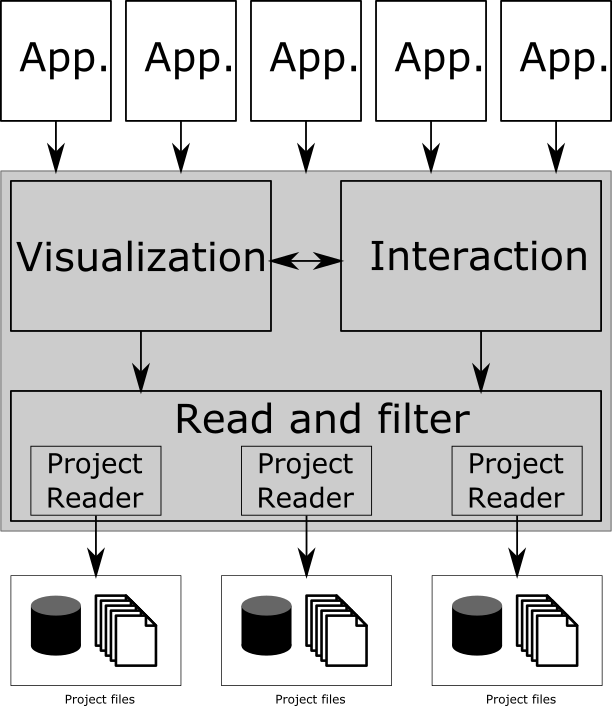
\includegraphics[width=0.6\linewidth]{figures/arquitecture.png}
\end{center}
 \caption{\label{fig_arch} The BRAVIZ software architecture}
\end{figure}


\subsection{Design and Development Methodology}

A ``user centered'' approach \cite{wassink_applying_2009} was used to design and implement BRAVIZ. The authors worked closely with brain researchers of several specialties, visited several labs and hospitals, and learned as much as possible about research workflows and the bottlenecks they contain. Prototypes were implemented in several iterations and shared with different domain experts, whose feedback motivated the design of the next generation.
The initial stages of design focused on identifying the obstacles that affect exploratory analysis and communication between experts, and examined ways of mitigating them. The team of experts was composed of radiologists, psychiatrists, physicians, neurophysiologists, pediatricians, statisticians, engineers and economists.
From analyzing the visualization options in current neuroimaging tools, as well as how domain experts used them, the BRAVIZ team learned what was expected from image viewers, i.e. which features were important to implement and which were seldom used. SPM \cite{friston_statistical_2007}, Osirix \cite{rosset_osirix:_2004} and 3D-Slicer \cite{fedorov_3d_2012} were the reference at this stage. For example, researchers needed to visualize several types of data in the same space and to be able to compare brain images between two subjects. Also obvious was the need to integrate spatial visualizations with non-spatial data for the same subject in order to be able to understand relationships. Another common need discovered in this exchange with expert users was the navigation from one subject to the other without having to re-start the visualization application per subject. This was satisfied by means of graphical user interfaces.


\subsection{Applications Set}


The current set of BRAVIZ applications can be divided in three categories. One set of applications measures or creates new descriptors from geometric data, one displays geometric data using other variables as context, and the third explores numerical and categorical data. This ensures different stages of the exploratory analysis process, respectively, data transformation, visualization and subjects-to-group analyses. Additional modules can import and export data in spreadsheet format to interact with numerical and categorical data. All tools  are accessible from the graphical menu shown in Figure \ref{fig_menu}

\begin{figure}
\begin{center}
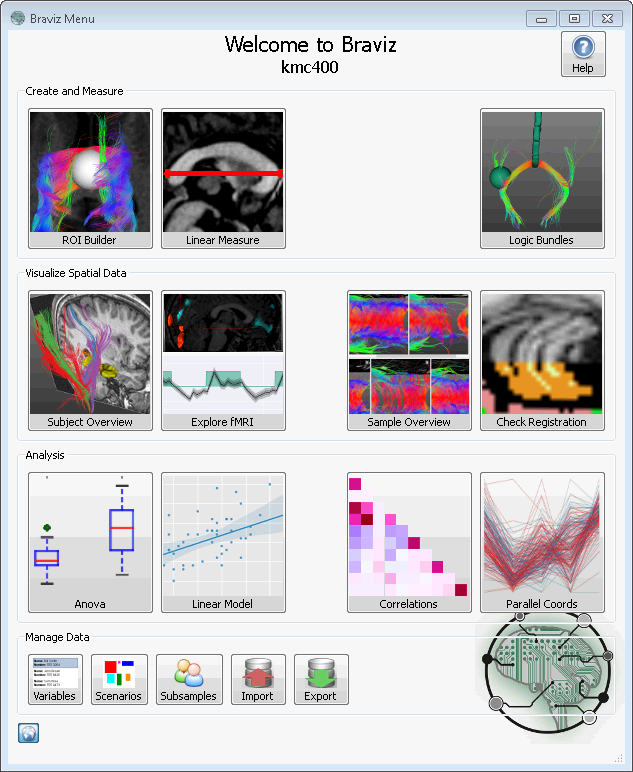
\includegraphics[width=0.4\textwidth]{figures/braviz_menu.PNG}
\end{center}
 \caption{\label{fig_menu} BRAVIZ main menu }
\end{figure}


\subsubsection{Descriptors for geometric data}

The ROI Builder application (Figure \ref{fig_roi}) provides an interface for helping experts position spherical ROI  (region of interest within brain) on each subject. These spheres are placed and sized with respect to images (from any modality) or cortex reconstructions. It is also possible to preview the fibers that cross the ROI, and then evaluate mean value inside the sphere of any scalar image, for example mean FA (fractional anisotropy) or mean T value associated with an fMRI test. 
Linear and non-linear registration maps can be used to approximate the position and size of the sphere in other subjects. The expected workflow is positioning the ROI in one subject, extrapolating it to a sample and correcting; and the interface was optimized to support it (buttons, hotkeys and visualization). Several ROIs can be used to select more complex bundles. All data generated in the application (ROIs, bundles and scalars) can be used on any other BRAVIZ application. 

In addition, the current BRAVIZ implementation includes an application for making linear measurements (lengths) of anatomical structures, and an application for defining fiber bundles by combining ROIs and segmented structures through logical operations.


\subsubsection{Geometric Data Visualization}

The Subject Overview application is shown in Figure \ref{fig_subject}. This tool  provides access to several kinds of spatial data in a unique 3D render and eases the rapid navigation from the data of one subject to another. Geometrical features such as MRI volumes or mean fractional anisotropy of DTI in relation to a specific structure can be captured directly from this application and added to the database as a new variable. The application also shows the values for selected variables per subject as well as annotations from the users. This ensures an integrated overview of each case depending on the data feeding BRAVIZ.

A display of small multiples \cite{tufte_visual_1983}  brain views  of several subjects is useful for finding trends across a sample or for quality control to detect contaminated images. Subjects are ordered from left to right according to a chosen numerical variable and each row corresponds to a nominal variable. In the example presented in Figure \ref{fig_sample}, the two rows are men and women, and the ordering variable is the score on a math test. The bar-plot at the right shows the distribution of the variable (math test scoring) amongst the two groups (men vs. women) and is linked with the 3D views. If a more detailed view of any subject is required, the user may right click on that subject’s image to load the corresponding subject on other BRAVIZ applications.

The fMRI Explorer application from Figure \ref{fig_fmri} displays raw BOLD signals and contrast designs associated to fMRI experiments. It can also be used to compare signals at different locations or from different subjects.



\subsubsection{Numerical and Categorical Data Exploration}

The ANOVA application (see Figure \ref{fig_anova}) provides direct access to these models implemented in \emph{R} \cite{team_r:_2012}. After fitting the model the main plot shows diagnostics (distribution of residuals and a scatter plot of residuals vs fitted values) for validating the ANOVA hypotheses (normally distributed noise with constant variance) and the table at the bottom right shows the resulting statistics. The application can also show box-plots and scatter-plots which provide additional insight on the relation between regressors (nominal and numeric variables and interaction terms) and outcome. Individual points in these plots may be identified by placing the mouse over them. Additionally, by right clicking, they can be loaded on other BRAVIZ applications to get additional information, this is especially useful for outliers.

Figure \ref{fig_lm} shows an alternative application which fits standard linear models and shows the effect of each regressor (numerical variables, dummy variables associated to a level of a numerical variable or interactions). The correlations application shown in figure \ref{fig_correlations} displays a list of variables, a correlations matrix of selected variables, and scatter plots of selected correlations. As usual, points in the plot can be queried and right clicked. Additionally, they can be temporary eliminated from the analysis to see the impact they have on the correlation. The parallel coordinates display from figure \ref{fig_parallel} provides another way of analyzing relations involving several variables.

\begin{figure}
\begin{center}
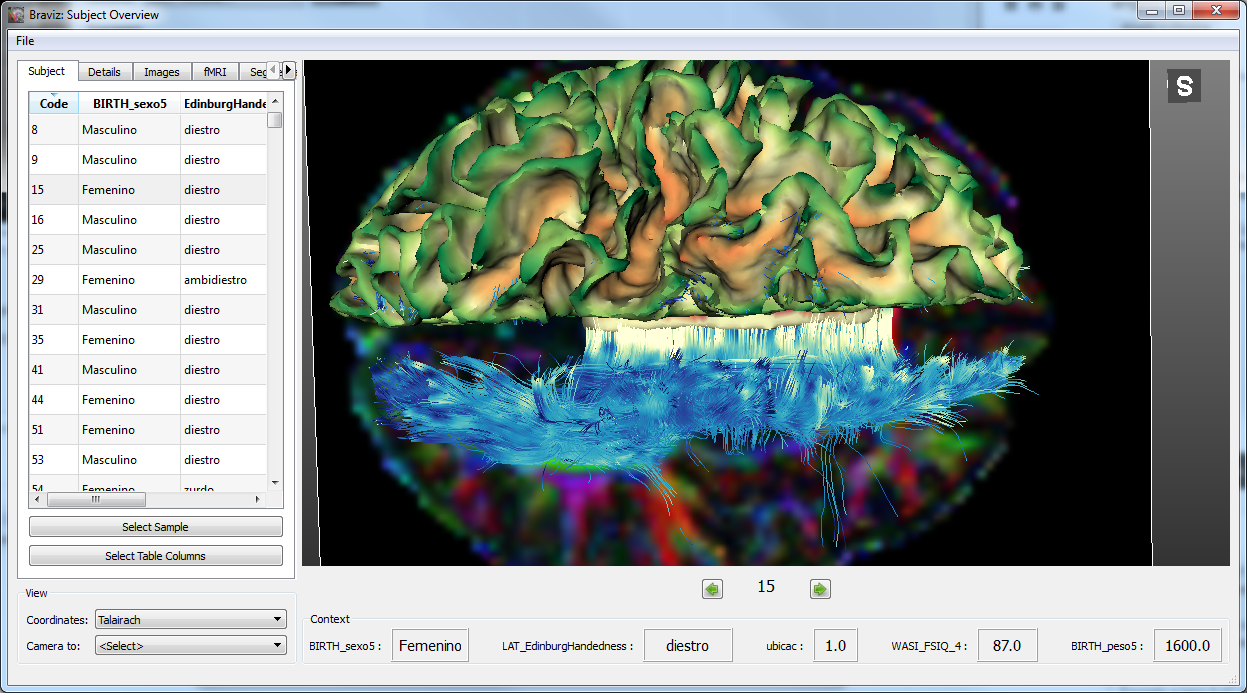
\includegraphics[width=\linewidth]{figures/subj_overview_full.PNG}
\end{center}
 \caption{\label{fig_subject}Main interface of the subject overview application: At the bottom of the render some variables about the subject provide context}
\end{figure}

\begin{figure}
\begin{center}
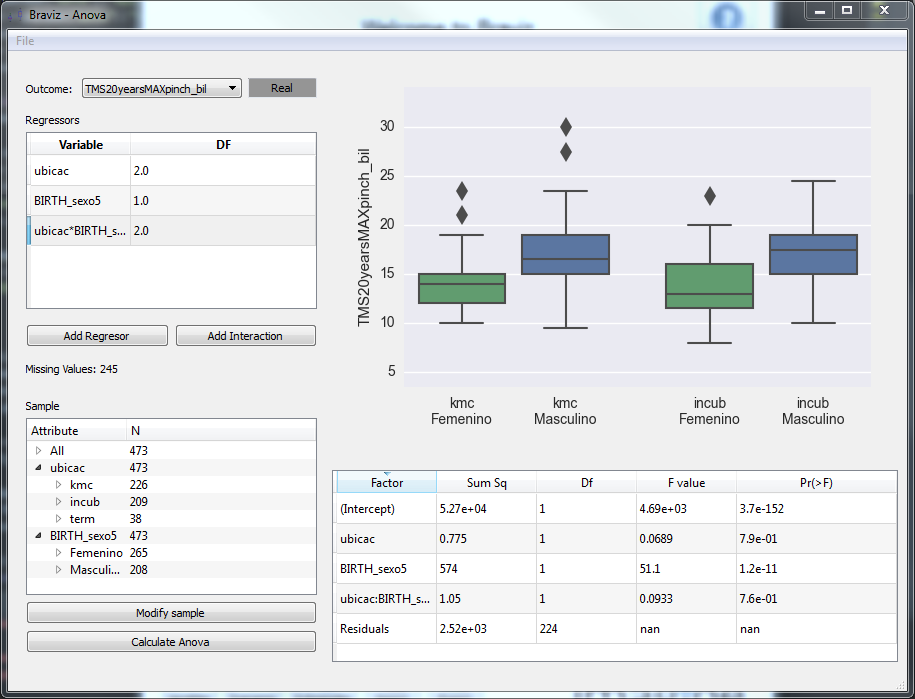
\includegraphics[width=\linewidth]{figures/anova.PNG}
\end{center}
 \caption{\label{fig_anova}An application for performing ANOVA analyses using the data in the BRAVIZ database.}
\end{figure}

\begin{figure*}
\begin{center}
\begin{subfigure}[b]{0.18\linewidth}
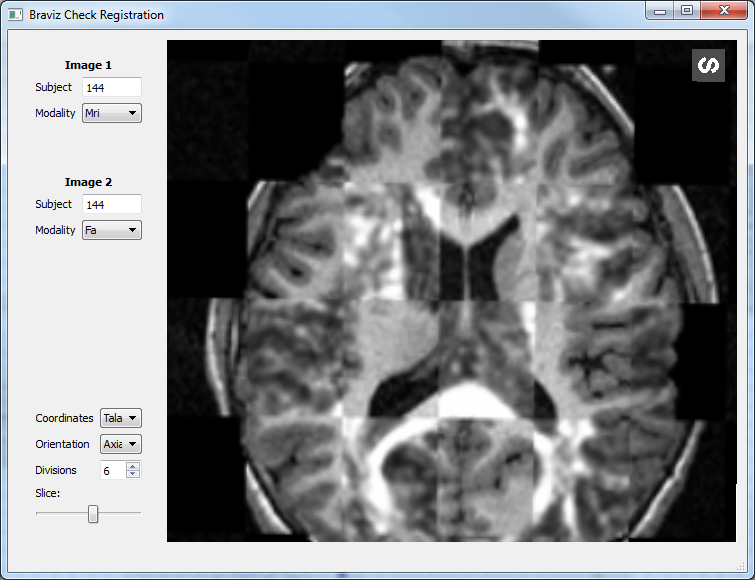
\includegraphics[width=\textwidth]{figures/check_reg}
\caption{\label{fig_check_reg}Check Registration}
\end{subfigure}\hfill
\begin{subfigure}[b]{0.3\linewidth}
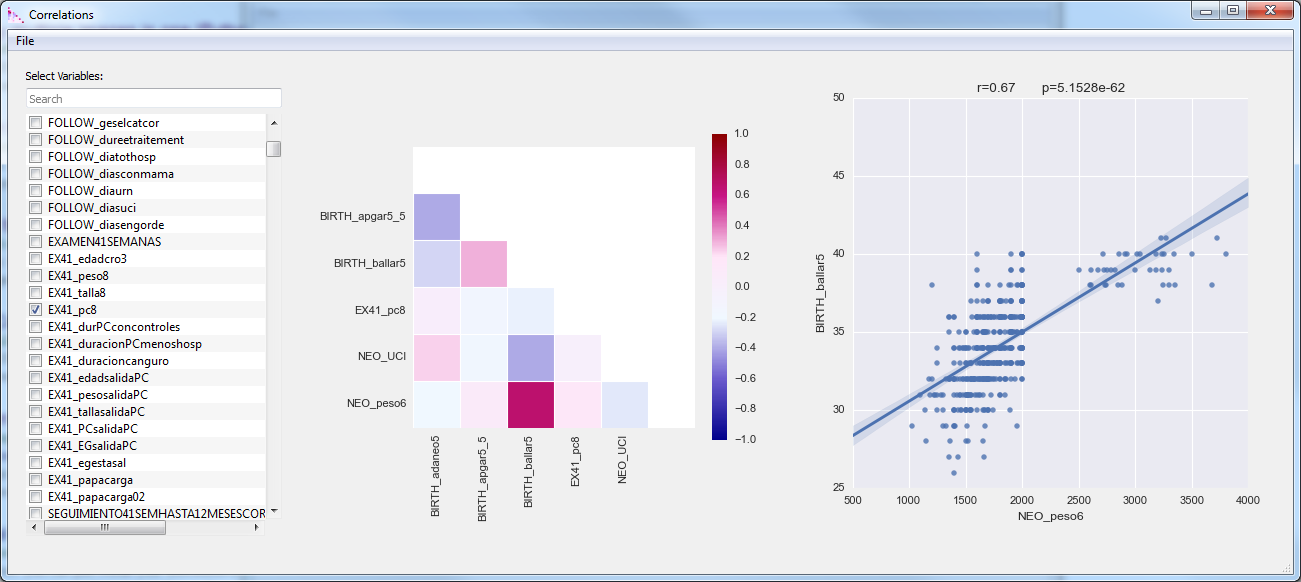
\includegraphics[width=\textwidth]{figures/correlations}
\caption{\label{fig_correlations}Correlations}
\end{subfigure}\hfill
\begin{subfigure}[b]{0.22\linewidth}
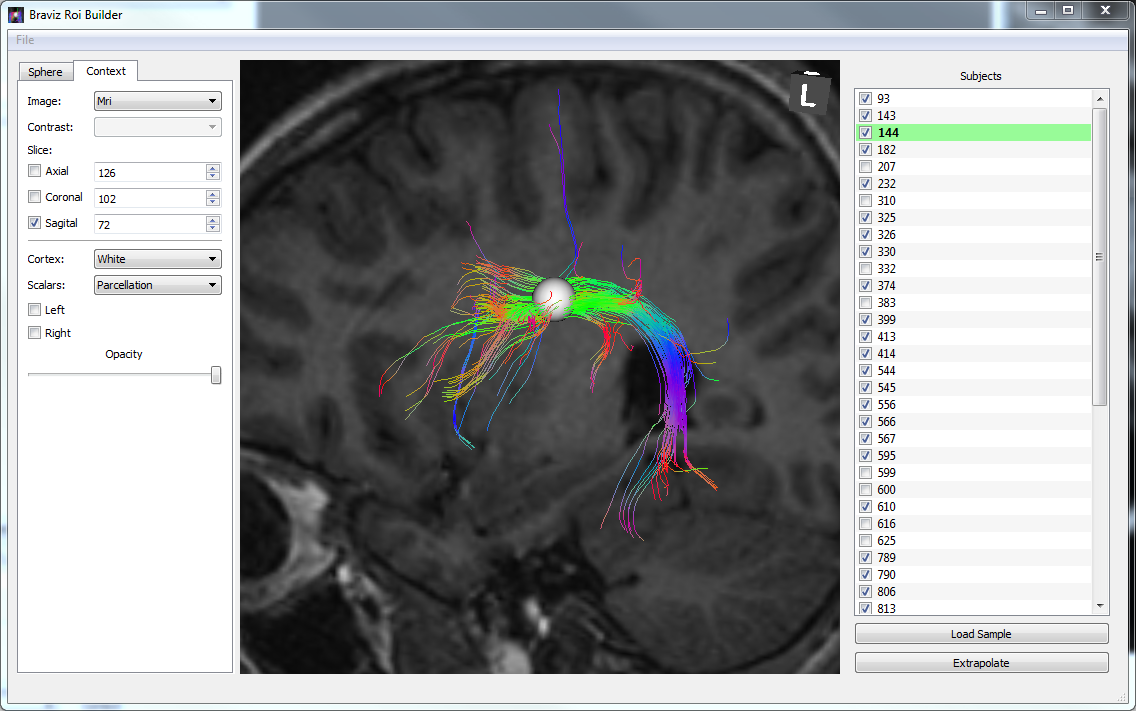
\includegraphics[width=\textwidth]{figures/roi_builder}
\caption{ROI Builder\label{fig_roi}}
\end{subfigure}\hfill
\begin{subfigure}[b]{0.18\linewidth}
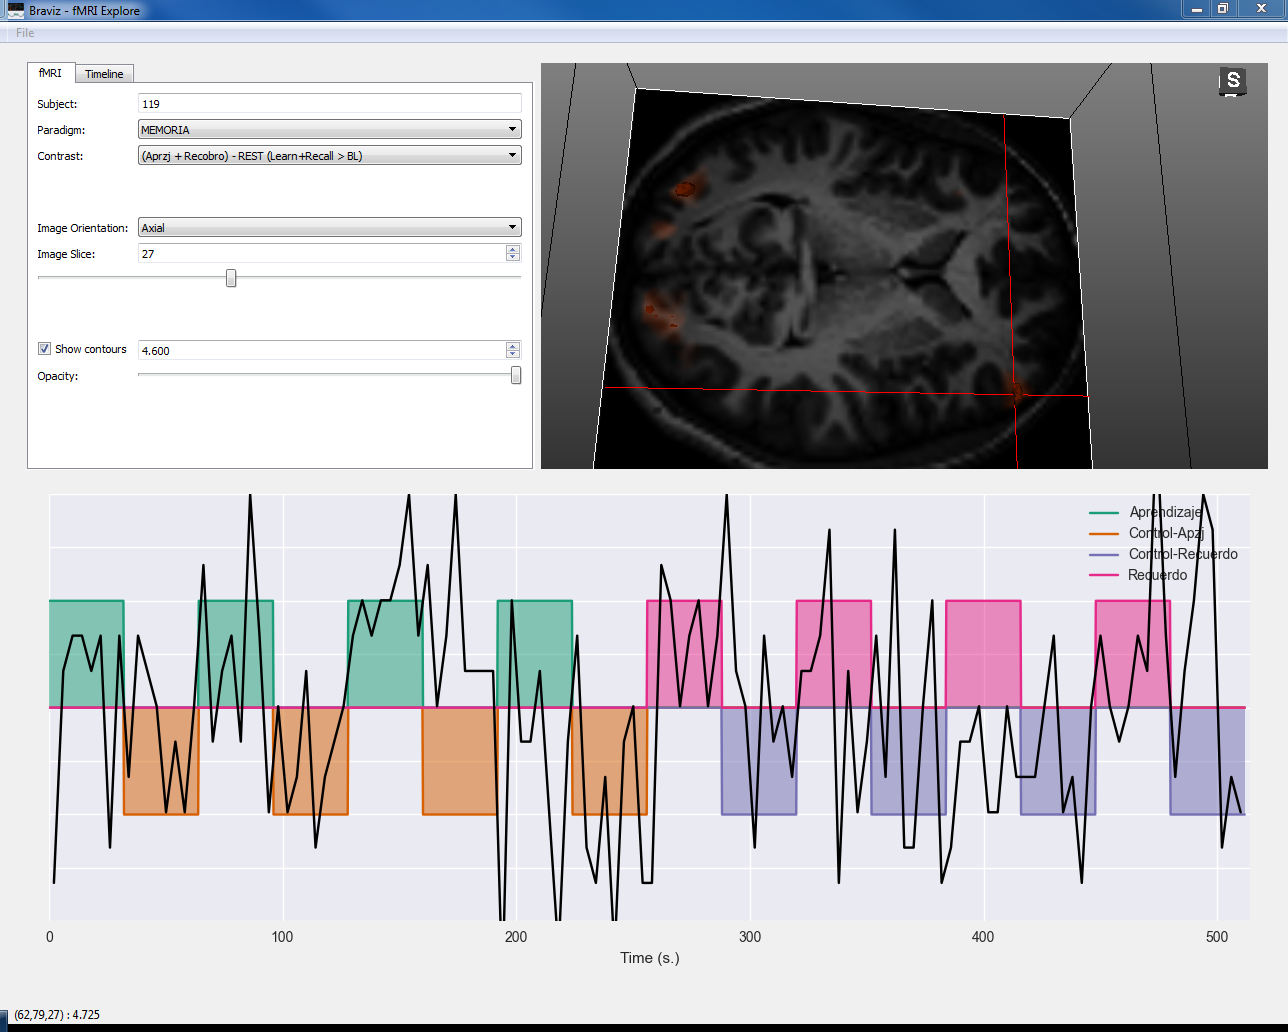
\includegraphics[width=\textwidth]{figures/fmri}
\caption{FMRI Explorer\label{fig_fmri}}
\end{subfigure}
\end{center}
 \caption{\label{fig_other_apps} Examples of BRAVIZ Applications}
\end{figure*}



\subsection{Global BRAVIZ Features}

In addition to the unique features of each BRAVIZ application, the whole tool provides features that directly support integrated exploratory analyzes. In addition, tools are designed to be used together and combined to complete complex analyzes.

\subsubsection{Linking Clinical and Structural Data}

Subjects in BRAVIZ are always considered as a whole, and therefore all of their associated data is always accessible. For example, the Subject Overview application displays a set of clinical variables and annotations together with spatial-data. This added context lets researchers make a more accurate reading of images and other spatial data. Using other tools, researchers would need to seek this information elsewhere. 

Several scalar measurements can be derived from spatial data within the tool itself. For example a group of segmented structures can be selected and their combined volume added as a new variable. These values can afterwards be used together with clinical variables for statistical analysis, but a link is kept between the data and the environment in which it was generated. Continuing with the example, if the researchers finds an outlier, he can right click on it and from the context menu open the application in which the value was generated, with the configuration it had at that time, but focused on the subject of interest. In this way it can be reviewed if the extreme value was caused by a particular structure of the subject, which could be an error in segmentation, a problem with the image, or sign of an actual pathology.

\subsubsection{Comparing Subjects}

A common task in exploratory research is analyzing similarities and differences amongst a group of subjects. Most existing visualization tools for spatial data force researchers to select the subject of interest at the very start, and then configure all the visualization options and load the necessary files. BRAVIZ takes a different approach, and always allows the subject to change at the middle of the analysis while maintaining the configuration of the application. In this way it is easy to look at different subjects from the same point of view, which makes comparing data very efficient.  

\subsubsection{Working with Samples}

Often some properties of the data will only apply to an specific group of subjects. In BRAVIZ samples are a central component of every analysis. The can be defined by using filters on variable values, manually adding and removing specific subjects, taking random subsets, or combining samples through set operations (union, intersection and difference). These samples can then be used throughout the tool, which makes repeating analyzes for different groups easy. They can also be modified, for example to remove pathological data points, and the results of the modification visualized in real time. In contrast, most tools oriented towards confirmatory research require the sample to be set at the start of the analysis.

\subsubsection{Supporting Long Workflows}

Analyzing a complex dataset requires a significant amount of time, will likely be spit in multiple sessions. In order to ease re-using previous work, BRAVIZ applications allow saving and restoring their state using custom names and descriptions, and attaching textual annotations to subjects, variables and geometric objects (for example ROIs). In addition, a log of each analysis session is kept, which can be reviewed and annotated using a web interface. These features also allow other researchers to understand the meaning of variables, geometric structures and scenarios created by colleagues; which fosters collaboration. 

\subsubsection{Integrating Tools}

In addition to the common database where all tools read and store variables and geometric objects, BRAVIZ includes a real time communication mechanism. Through it, all applications can be coordinated to focus on the same subject (see Figure \ref{fig_imagine}), work with the same sample, or use the same set of variables. Applications may be running on different screens or even different devices; allowing researchers to get different perspectives of the data just by moving their eyes.

\begin{figure}
\begin{center}
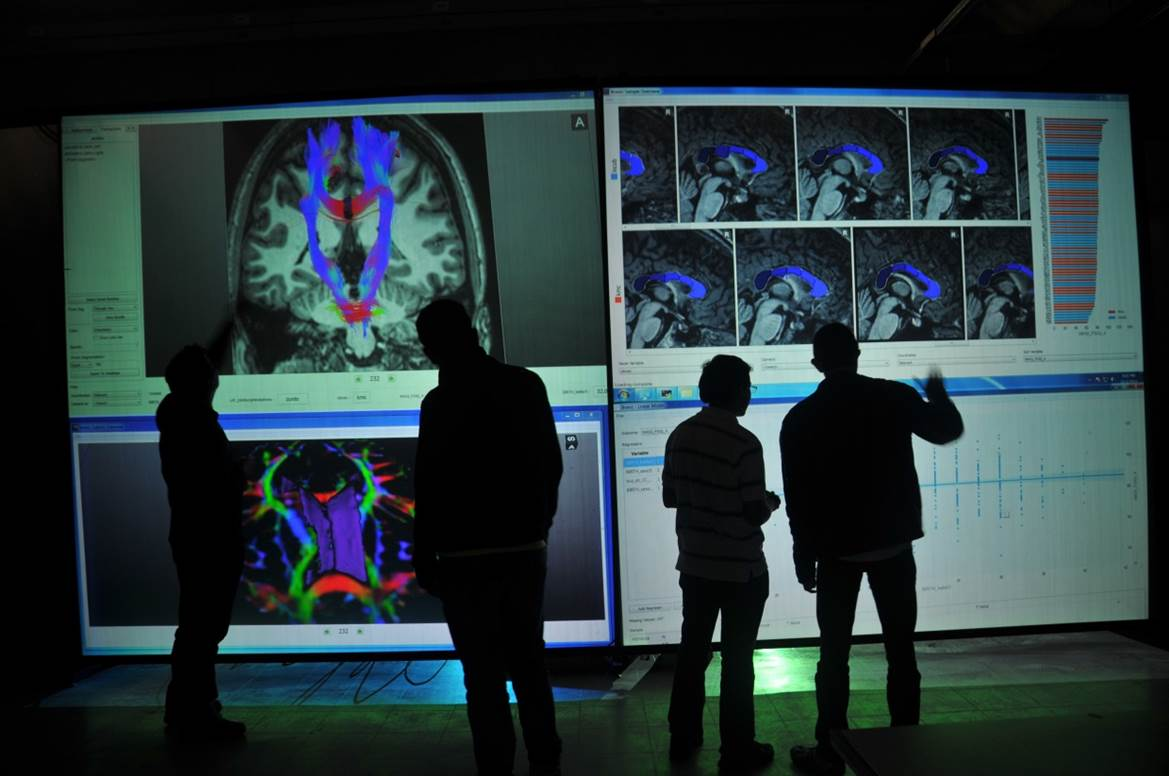
\includegraphics[width=\linewidth]{figures/imagine.jpg}
\end{center}
 \caption{\label{fig_imagine} An example of BRAVIZ running on a large display in a collaborative setting.}
\end{figure}

\section{Case Studies}

In this research, a particularly representative case study, the KMC (Kangaroo Mother Care) project, is introduced to both motivate the requirements for BRAVIZ and demonstrate its effectiveness. An original randomized study involving around 750 preterm babies was conducted in 1994 \cite{charpak_kangaroo_1997}. These children were followed during their first year \cite{charpak_randomized_2001}, \cite{tessier_kangaroo_2009} of life and several clinical and socio-economical variables were registered. Forty of these children were re-located later at fifteen years of age, and they were submitted to several neuropsychological tests, measuring attention, memory, reasoning skills and hand-eye coordination among others. They also had vision, hearing, and TMS tests\cite{schneider_cerebral_2012} and full medical examinations . Finally, they were scanned with Structural MRI, DTI (Diffusion Tensor Imaging) and several functional MRI (FMRI) paradigms. These images were processed with Freesurfer \cite{fischl_freesurfer_2012}, fsl\cite{jenkinson_fsl_2012}, camino\cite{cook_camino:_2006}, and spm\cite{friston_statistical_2006}; which extracted several numerical measurements and geometric structures like segmentation and tractography. All of this data was collected for testing specific hypotheses but the specialists involved in the study are also interested in analyzing it for unexpected relationships and trends; in other words, to perform exploratory analyses.

\subsection{Relations between fibers and Neuropsychological}

One of the applied tests was the WISC (Wechsler Intelligence Scale for Children), which is divided in four indices: Verbal Comprehension, Perceptual Reasoning, Working Memory and Procession Speed. 	Language capacities are known to be associated with the posterior area of the corpus callosum, which can be analyzed in the KMC dataset. 

The first task is extracting an appropriate measurement for the quality of the anterior area of the corpus callosum (CC), which can be accomplished using the subject overview application. In the segmentation tab, the anterior and mid anterior sections of the corpus callosum can be selected. In this tab it is possible to calculate the volume or the mean FA (Fractional Anisotropy) inside these regions. However, in order to get a more robust measurement, the tractography panel can be used to calculate the fibers that go through these regions. Then, the mean FA, mean length and number of streamlines in this bundle can be calculated. All of these measurements are correlated between them, but the length of the fibers includes more information of the region, as streamline propagation is controlled by an FA threshold, consistent high FA values around the CC will cause streamlines to grow longer.

After calculating this measurement, the relationship can be visualized using the Linear Model application. This initial plot is shown on Figure \ref{fig_lm}.

\begin{figure}
\begin{center}
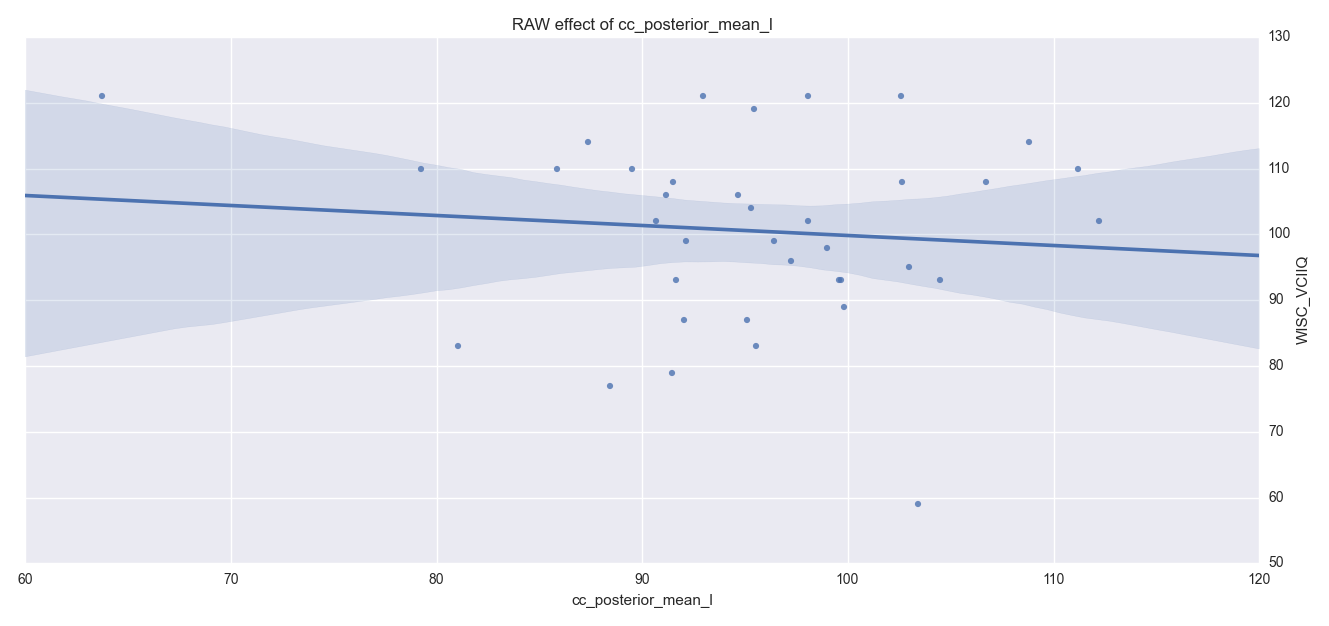
\includegraphics[width=\linewidth]{figures/cases/initial_corr}
\end{center}
 \caption{\label{fig_lm}An initial correlation with a prominent outlier}
\end{figure}


It is clear that the point at the extreme left is an outlier which has to be analyzed in more detail. By right clicking on it, a context menu appears with the option of opening the respective subject on the Subject Overview Application, with the visualization used for calculating the measure. This view is shown on Figure \ref{fig_subject2}, compared to a term subject in the middle of the plot.

\begin{figure}
\begin{center}
\begin{subfigure}[b]{0.48\linewidth}
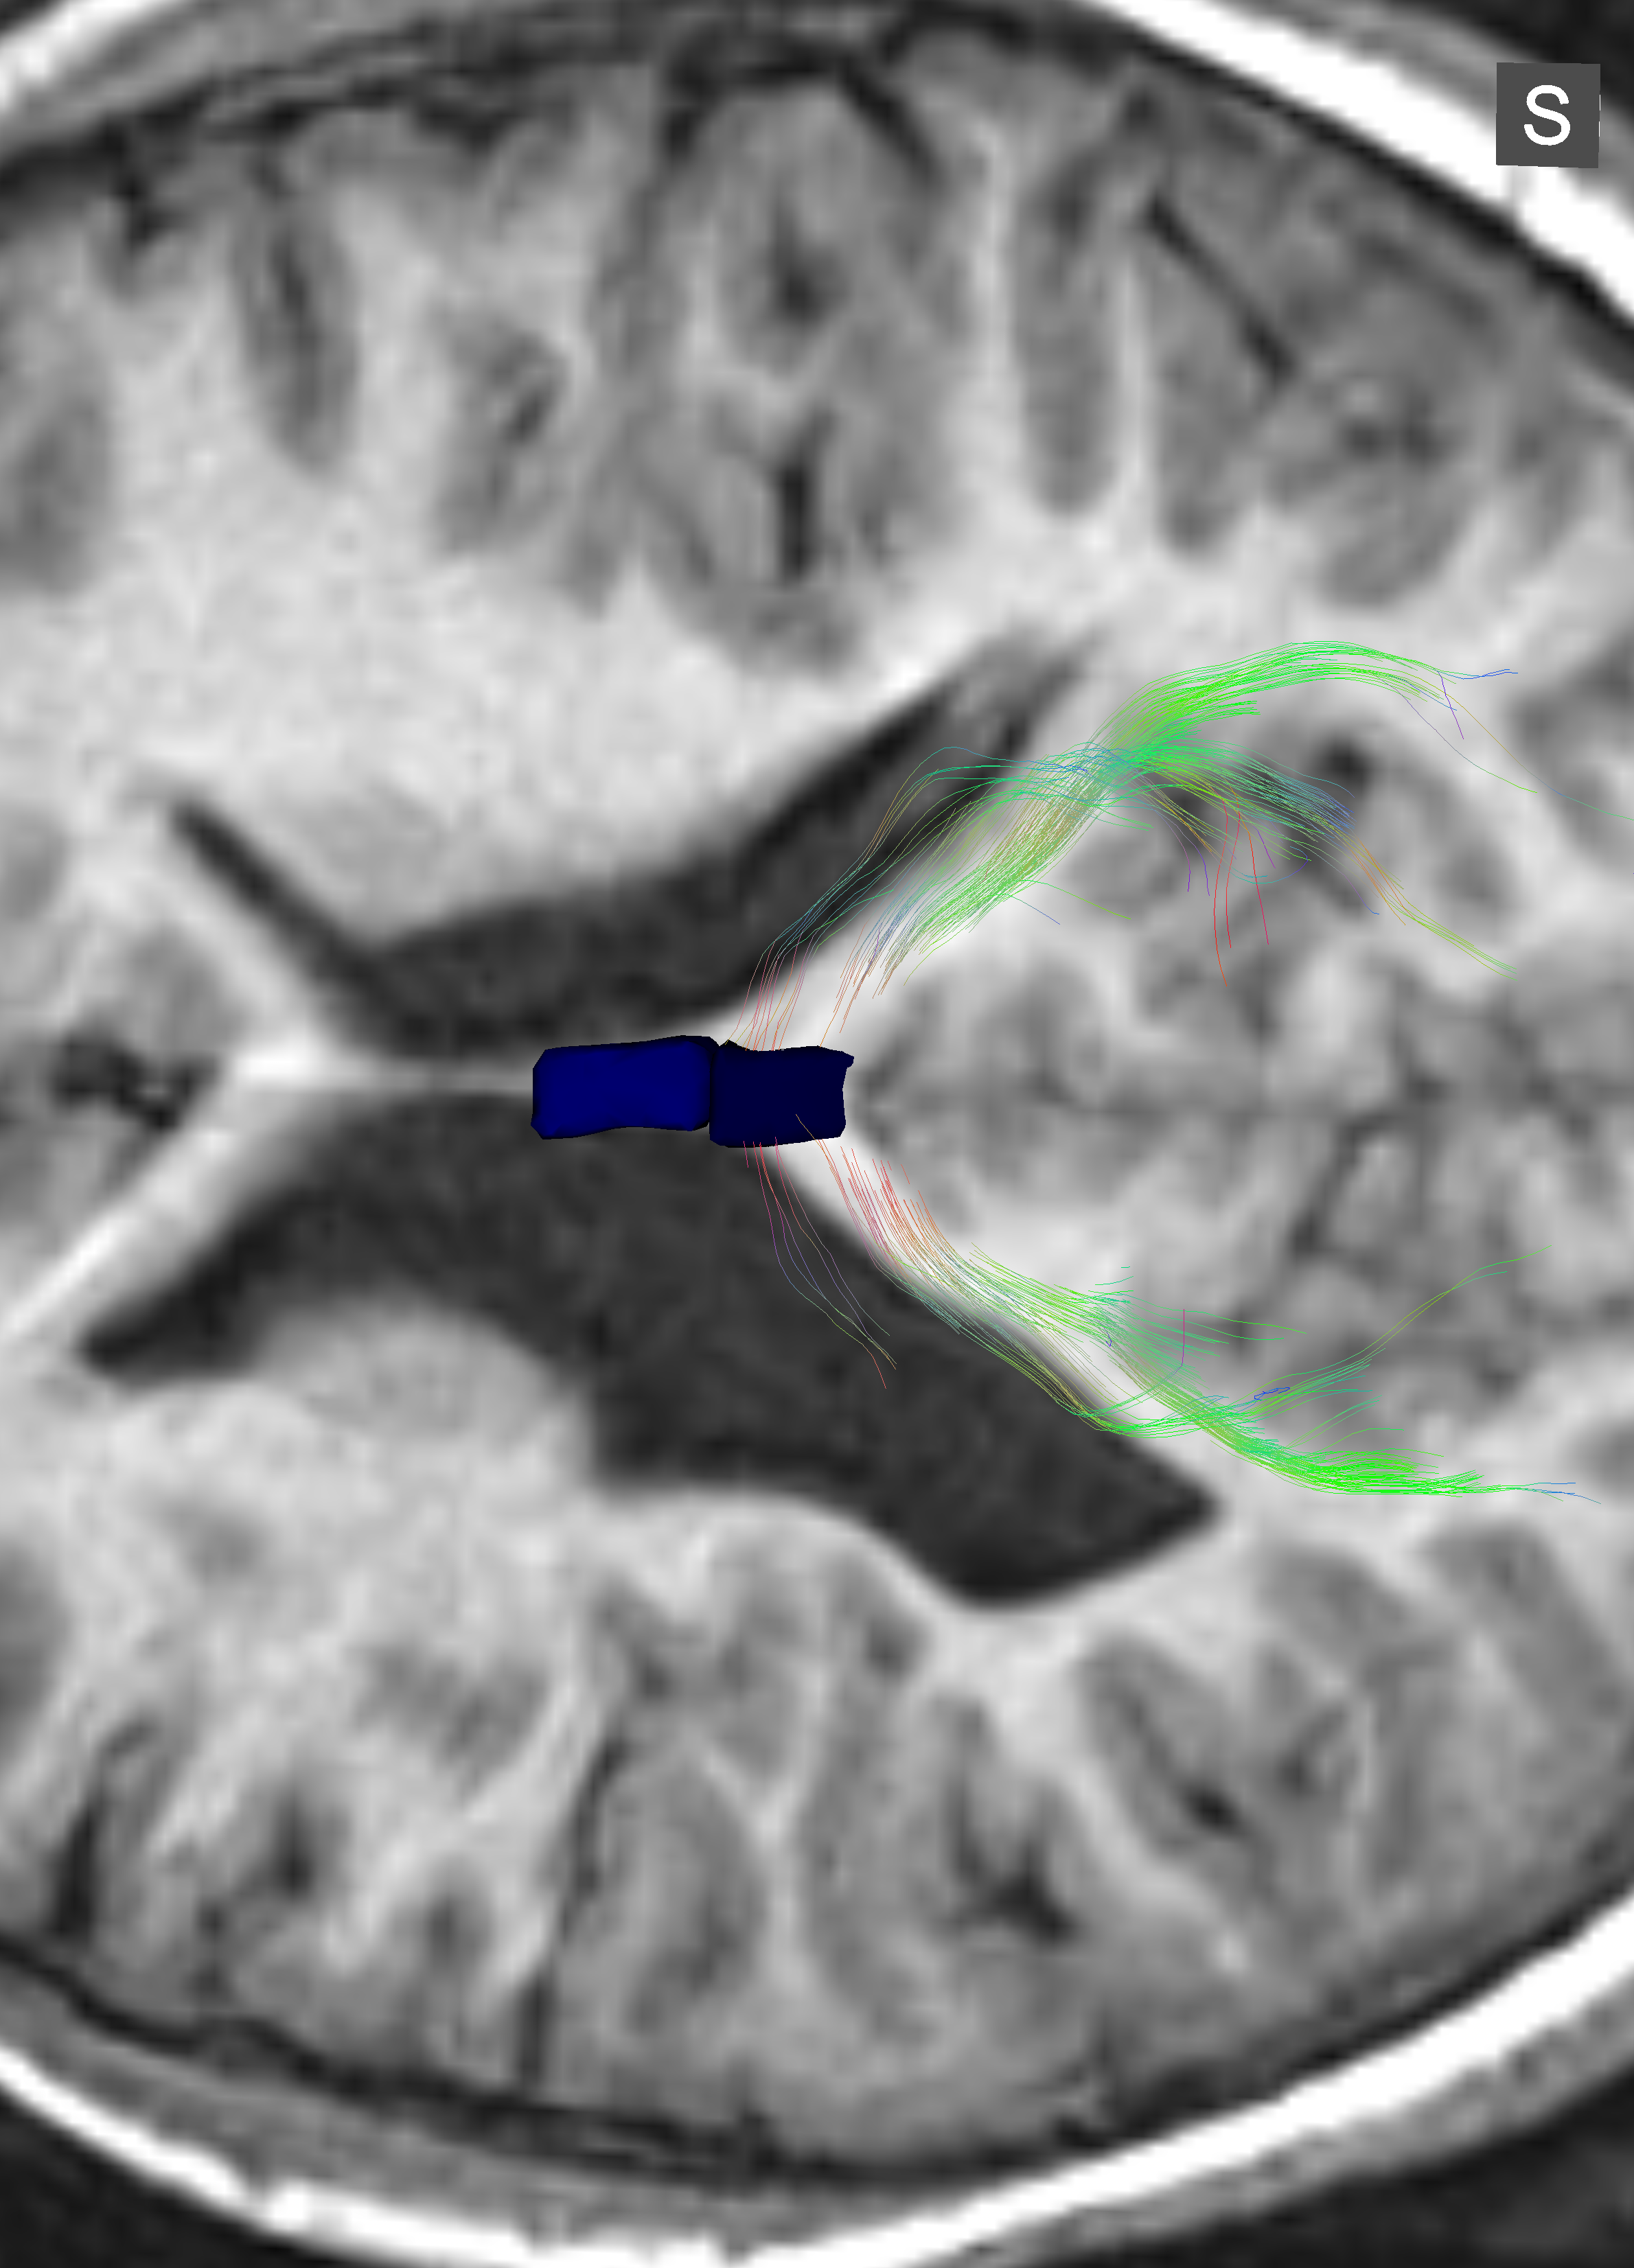
\includegraphics[width=\textwidth]{figures/cases/cc_fibs_posterior_outlier}
\caption{\label{fig_cc_outlier}outlier}
\end{subfigure}\hfill
\begin{subfigure}[b]{0.48\linewidth}
\includegraphics[width=\textwidth]{figures/cases/cc_fibs_posterior_control}
\caption{\label{fig_cc_control}control}
\end{subfigure}
\end{center}
 \caption{\label{fig_subject2} Posterior Corpus Callosum Fibers from the outlier from Figure \ref{fig_lm} compared to a control subject}
\end{figure}

The MRI image has significant noise, and there are several missing fibers in the corpus callosum. This is an unfortunate problem associated to data acquisition that cannot be corrected by the tool. Therefore this point must be excluded from the analysis. At this point it is worth asking if there are more subjects with similar data quality problems. To check this, the whole sample can be loaded in the Sample Overview application, in a view that shows the corpus callosum and associated fibers (Figure \ref{fig_parallel}).

\begin{figure}
\begin{center}
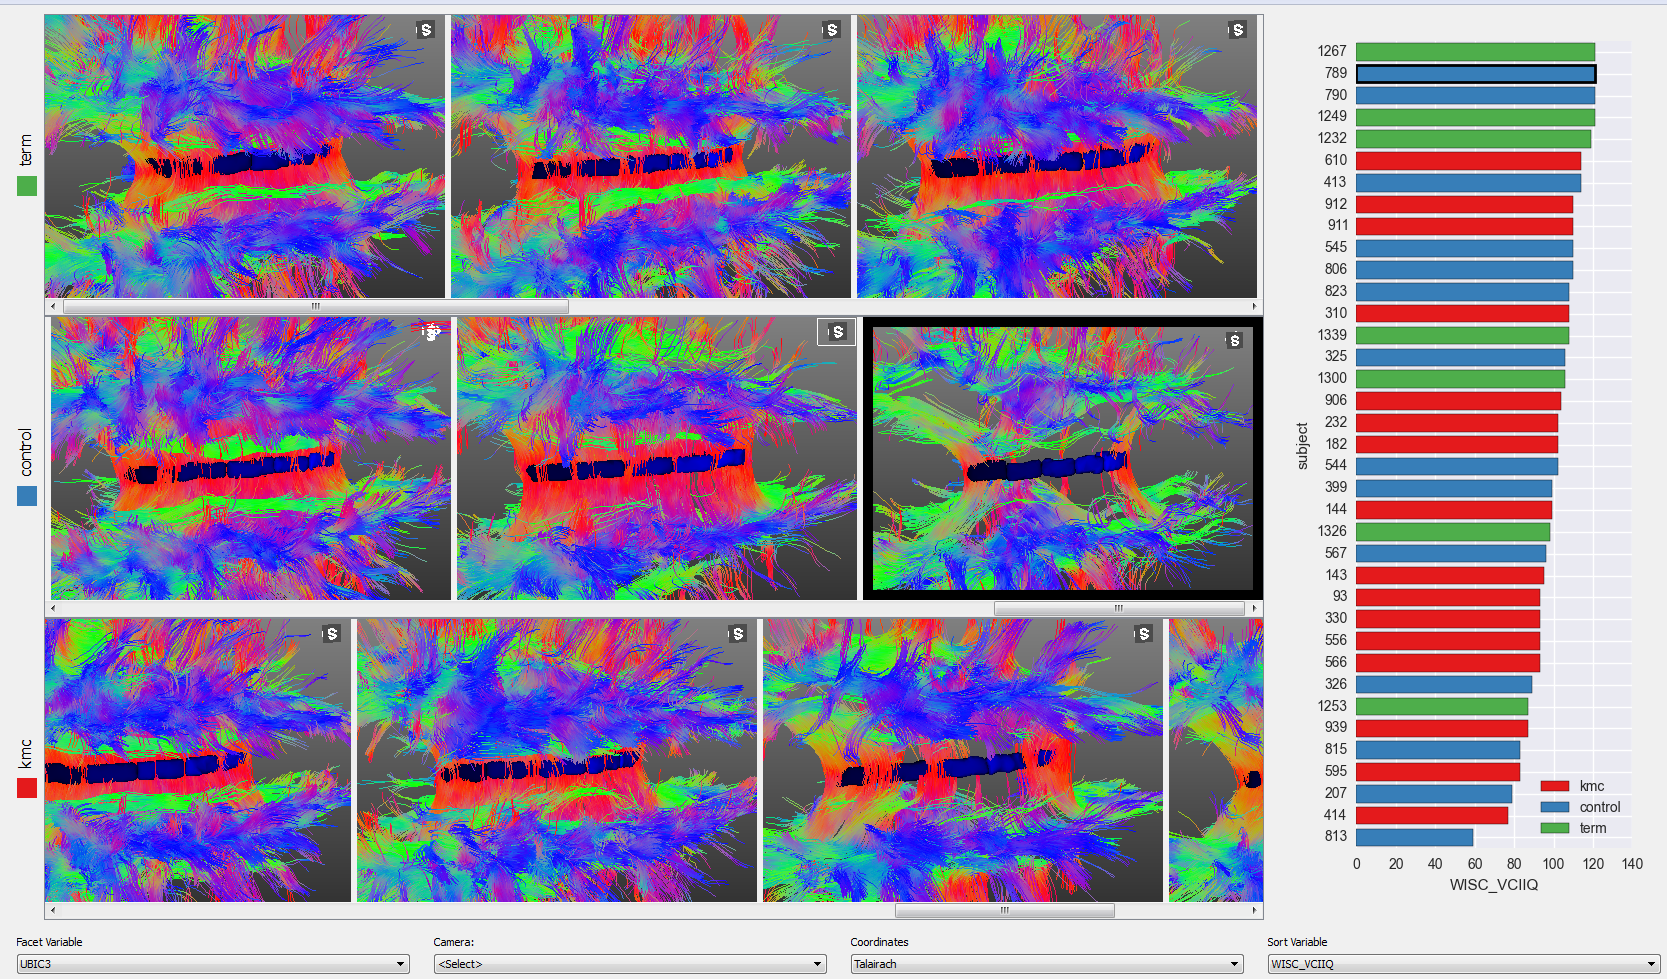
\includegraphics[width=\linewidth]{figures/cases/quality_control_trim}
\end{center}
 \caption{\label{fig_sample} Quality control on the corpus callosum fibers from the whole sample}
\end{figure}

From this view, some additional subjects with fiber tracking issues are detected and excluded from the sample. The corrected sample (28 subjects) can then be shared with the Linear Model application which updates the plot to the one in Figure \ref{fig_lm2}.


\begin{figure}
\begin{center}
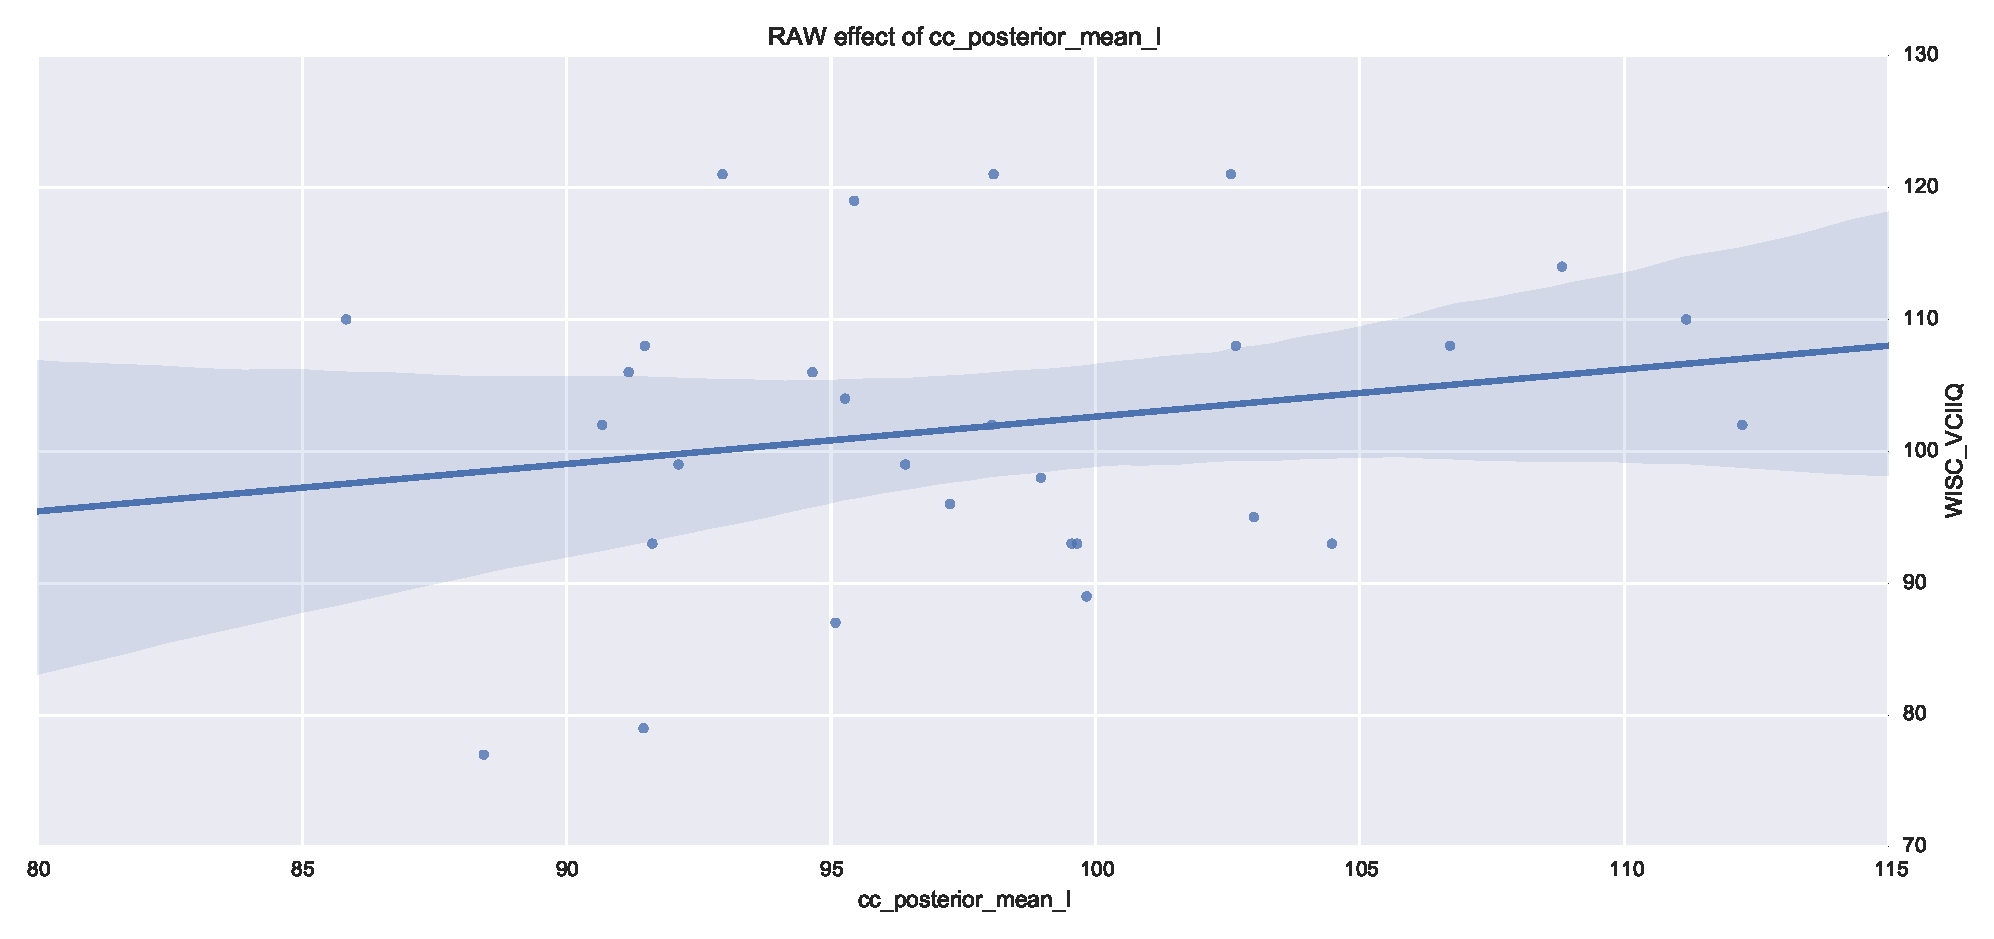
\includegraphics[width=\linewidth]{figures/cases/final_corr}
\end{center}
 \caption{\label{fig_lm2} Correlation from figure \ref{fig_lm} with corrected sample}
\end{figure}


This plot shows a slight correlation between the lengths of the fibers that go through the posterior part of the CC with the Verbal Comprehension Score. By fitting the actual model it can be seen that it has an associated P value of 0.28; which is not significant, but is good enough to try testing this hypothesis in a larger dataset.
  

\subsection{Searching for a Pathology}

Periventricular leukomalacia (PVL) is characterized by a lesion in the periventricular germinal matrix, which results in a loss of white matter and a compensatory growth in the ventricular system. Preterm babies, especially those born prior to 33 weeks of gestation, have a significant risk of suffering from this condition, which can cause motor and vision problems, cerebral palsy and epilepsy.    
The images in this study were not analyzed for this condition, and the imaging protocol did not include FLAIR images, which are the most appropriate for detecting PVL. However has other data that can be used to search for subjects who suffer from PVL.

A parallel coordinates display can be used to view the volume of the ventricular system and the total white matter. The possible effects of the condition would be lower scores in motor and visual tests and general intelligence assessment; which can also be added to the display. In addition, the dataset includes a neurological motor assessment which classifies subjects in normal and not-normal.  Finally the risk factors, weight and gestational age (Ballard) at birth, can also be added to obtain the display shown in Figure \ref{fig_parallel}.

\begin{figure}
\begin{center}
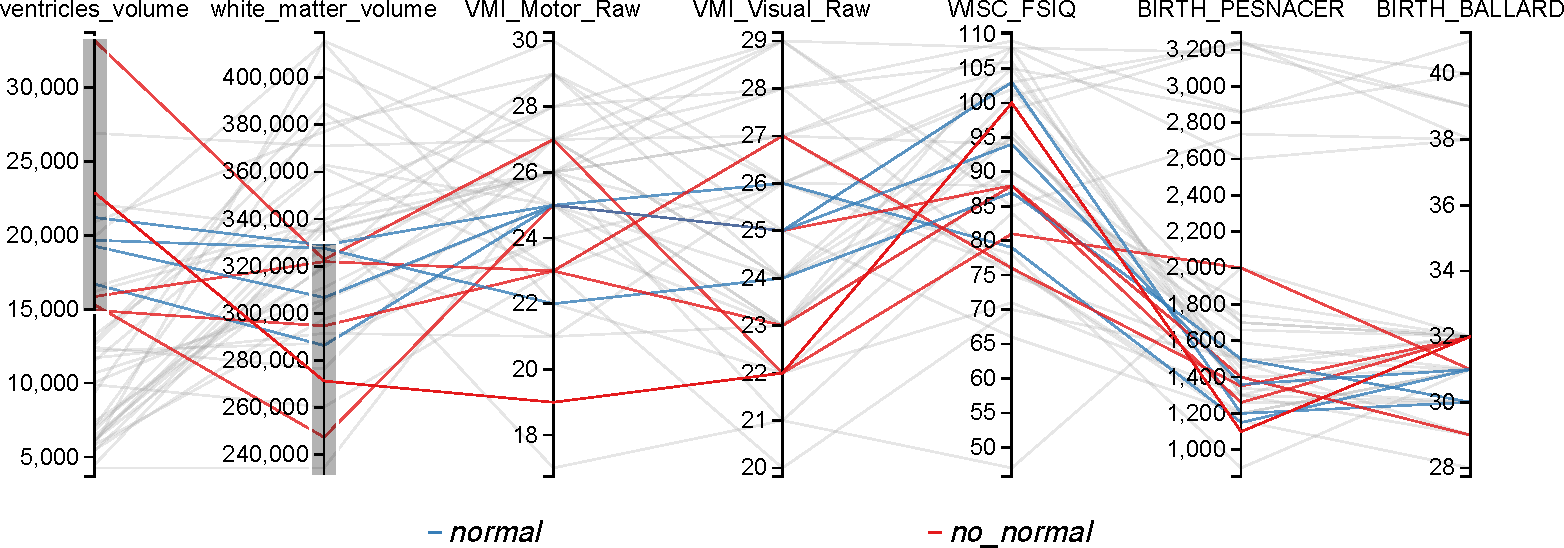
\includegraphics[width=\linewidth]{figures/cases/parallel_coordinates}
\end{center}
 \caption{\label{fig_parallel}Parallel coordinates display configured for searching PVL cases}
\end{figure}

Data in the visualization can be filtered by dragging on any of the axes, in this case only subjects with high ventricular volume and low white matter volume are kept. Two of the lines from the first segment of the graph have a distinctive downwards slope, which could indicate a dilation of the ventricular system which compensates a decrease in white matter, both of them have a not normal motor neurological exam. By hovering the mouse over each line they are highlighted, which allows to see that both of them have a low visual VMI score. By right clicking on any line a context menu appears which permits switching focus to the respective subject on other BRAVIZ applications to get additional details. 

By loading the subject associated to the top line in Subject Overview it is confirmed that he has a complicated perinatal history: C-section in emergency because of profuse bleeding (placenta previae) at 31 weeks of gestational age ( very premature infant). The  CT scan showed signs of leucoencephalopathy  and an  increased volume of the left lateral ventricle. His neurological examination showed normal psychomotor development. At 15 years, he presents an epilepsy in  treatment, severe bilateral hearing loss and abnormal bilateral vision.  

The subject associated to the highlighted line in Figure \ref{fig_parallel} was also born by C-Section in emergency. It was a twin pregnancy, the mother had HELPP syndrome (malignant hypertension) and died after giving birth. The neurological examination during the first year of life is abnormal, diagnosis of cerebral palsy at the end of the first year with spastic diplegia of inferior members and hemiparesia of the right arm.  There is a severe myopia corrected with glasses. All of these symptoms can be associated with PVL, the T1 Image appears to show white matter lesions typical of PVL (Figure \ref{fig_subject3}).

Two cases of PVL were successfully located in the sample first by looking at indicator variables and then looking at the details of the most likely candidates. Note that the details view in the Subject Overview applications contains all the required information to  understand each case, there was no need to search additional files. 

\begin{figure}
\begin{center}
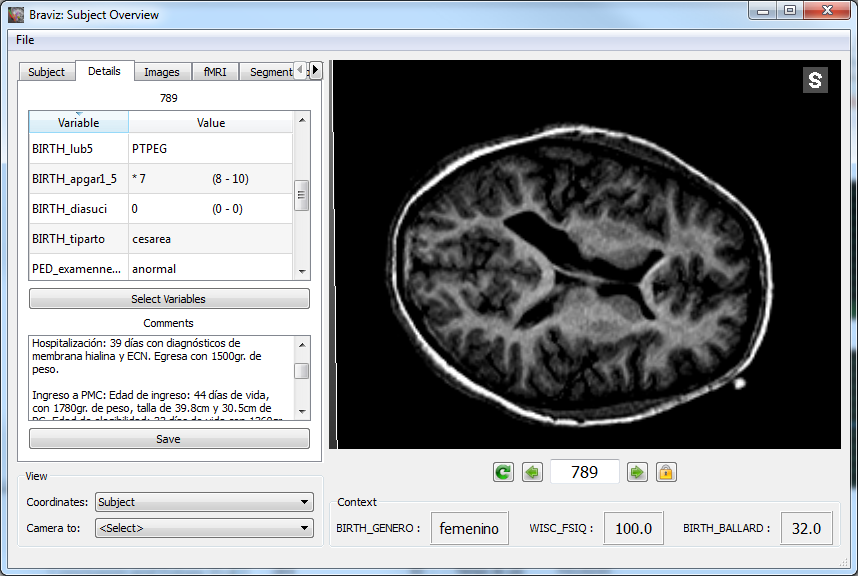
\includegraphics[width=\linewidth]{figures/cases/pvl_details}
\end{center}
 \caption{\label{fig_subject3}Details of a subject with possible PVL, the left panel shows values for several variables as well as the full clinical history.}
\end{figure}

\section{Discussion}
\label{sec:disc}

The presented cases illustrate how BRAVIZ can be used to increase understanding of a real data-set. 
It allows researchers to directly access all data, letting them explore it efficiently and retrieving data relevant to their questions. By combining several tools, users can perform group level analyses without losing track of individual subjects, and getting additional details from an interesting subject requires only one click. Sharing samples, variables, visualizations and subjects of interest also provides an efficient channel for experts to communicate and share ideas, thoughts and opinions with each other.

By providing direct access to all data BRAVIZ can help save time, but more importantly, it enables researchers to efficiently pursue all questions that come to mind. If finding the answer required a cumbersome procedure and gathering data from several sources, the question would not be explored unless it was a strong reason to do it. By easing data access, more questions can be explored which increases the chances of finding unexpected interesting results.

As most real datasets, the one considered here is not perfect and some data errors will always be present. Researchers should always have access to raw and processed data so that they can be certain of the veracity of results. This data should be rapidly accessible so that researchers can spend more time exploring data and not performing quality controls. When pathological data is found, they should be removed from analysis, annotated or fixed. Presenting data visually makes extreme values salient, for example values in different units or with a misplaced decimal point. Variable selection dialogs also give the subject the opportunity to review and fix variable meta-data (description, labels, range). The database can also be enriched by deriving measures from geometric data (automatically or with manual intervention) or importing additional variables from spreadsheets. Therefore the database evolves and becomes more valuable at each analysis round. 

Combining clinical and geometric data with the unstructured clinical history allows researchers to reconstruct a full picture of each subject. This is valuable for making accurate interpretations of results, for understanding the dataset and for deciding if a certain subject should be or not included in the sample of a certain analysis. Subjects in BRAVIZ always keep all their associated data, and therefore can always be analyzed as a whole.

Subjects can be isolated from groups to perform detailed case analysis, or attempts can be made to generalize the properties of a particular subject and often there will be iterations in both directions. BRAVIZ naturally support these movement from group to subject and back again.

It was also clear that the tools permit searching for subjects with specific conditions and isolating them for further analysis.
BRAVIZ provides several tools for manipulating samples, by applying filters, adding or removing individual points and combining several samples using set operations. These samples can be either saved into the database for future use or used instantaneously in statistical models or group data visualizations. Researchers can thus iterate through several samples, several models, several measurements and several views very quickly, thus gaining understanding of the data-set and raising questions and hypotheses for future projects.

A log of each analysis session which includes actions performed on different applications is automatically kept. These logs can then be revisited using a web interface. Researchers can enhance the log by labeling the most important steps and adding textual annotations. The state of an application at any point can be reloaded through a button, which allows researchers to revisit important visualization and explore different analysis paths. 

\section{Conclusions and Future Work}

BRAVIZ was designed as a tool for exploratory analysis of datasets which combine clinical and neuro-image data. Instead of a single application, it is implemented as a set of applications which can be used at different points of exploratory analysis, possibly by different members of the team. Some applications are designed to extract scalar measurements from image data, others provide detailed views of particular subjects or data types and others perform group analyses. Custom samples of subjects can be defined and used across all applications to focus the analysis. When several applications are running together, all of them can keep focus on the same subject, as shown on Figure \ref{fig_imagine}, which provides multiple points of view of the same subject that helps to understand how the different dimensions interact with each other. 

Even though the cases presented relied on a particular dataset, the architecture (Figure \ref{fig_arch}) of the tool was designed with portability in mind. All access to spatial data (images and derived objects) is performed inside a single module which provides a high level interface to the upper components of the system. By implementing several of these modules, the system can work on top of several projects which may have different mechanisms, layouts and formats for storing spatial data. Currently the system has been tested on a larger project from the Kangaroo Foundation which includes about 450 subjects, more complex fMRI paradigms, higher amounts of clinical data, and more anatomical imaging modalities.  

The architecture was also designed to make implementation of additional applications easy and to keep all low level data manipulation operations in a shared library. Thus, in the future more analysis tasks will be supported by specific applications. Several researchers have also expressed their interest in integrating other kinds of data, for example EEG signals or connection graphs \cite{rubinov_complex_2010} derived from DWI or fMRI. 

Currently there is a tendency towards moving data storage and processing to dedicated servers and providing access to users via web browsers. This allows researchers to work from any place, or even start a session on one place and finish elsewhere. Logs, variables, samples and other analysis artifacts could also be kept in a central location and therefore users could search for them in a single place. In addition, if multiple experts used the same back-end, sharing would become even easier. Note that the back-end could be a set of dedicated servers, or it could run in a scalable cloud. Powerful on demand data processing algorithms could also be provided leveraging high performance computing infrastructure. 

BRAVIZ needs to be tested in more datasets by researchers in other groups. The tool is licensed under a LGPL license and the source code is available at \url{diego0020.github.io/braviz}. The authors are willing to provide assistance to any interested party to set up the environment and start using it. 

As the tendency of collecting data in an open fashion and making it available to the general community grows, visual exploratory analysis tools like BRAVIZ and INVIZIAN will become more important. Acquiring data will no longer be a bottleneck for research, and a larger effort can be invested in analyzing existing data. This will lead to an increase in productivity of scientists everywhere, as well as a more optimal use of collected data, which summed up will increase the speed at which knowledge is generated.

\begin{acknowledgements}

This work was made possible by the Kangaroo Foundation. They generously provided a rich dataset, and the experts who work at the foundation were always willing to test prototypes and provide valuable feedback. The project also received important support from Colciencias, Universidad de los Andes, Iowa State University and CHUL.

\end{acknowledgements}

\bibliographystyle{spmpsci} 
\bibliography{zotero}


\end{document}
